\title{Лекция 12\\Представление в базе знаний предметных областей}
\author[]{Шункевич Д.В.}
\institute[]{Белорусский государственный университет информатики и радиоэлектроники}

\begin{frame}
	\titlepage
\end{frame}

\begin{frame}{\\Содержание лекции}
	\topline
	\justifying
	Понятие знания, типология знаний. Понятие предметной области, структурная спецификация предметной области, роли понятий в рамках предметной области. Понятие частной предметной области, родственной предметной области, виды частных предметных областей. Различные виды иерархии предметных областей, пересечения предметных областей.
\end{frame}

\begin{frame}{\\Понятие знания}
	\begin{SCn}
		\scnheader{знание}
		\begin{scnrelfromset}{свойства}
			\scnitem{синтаксическая целостность}
				\begin{scnindent}
					\scnrelfrom{пояснение}{корректность}
				\end{scnindent}
			\scnitem{семантическая целостность}
			\begin{scnindent}
				\scnrelfrom{пояснение}{смысл}
			\end{scnindent}
		\end{scnrelfromset}
	\end{SCn}
\end{frame}

\begin{frame}{Классификация знаний}
	\begin{SCn}
		\scnheader{вид знаний}
		\scnidtf{класс знаний}
		\scnhaselement{задача}
		\scnhaselement{спецификация}
			\begin{scnindent}
				\scnidtf{семантическая окрестность}
			\end{scnindent}
			\begin{scnindent}
					\scnsuperset{параметрическая модель}
					\scnsuperset{семантическая окрестность}
						\begin{scnindent}
							\scnidtf{набор свойств, которые описывают сущность}
						\end{scnindent}
					\scnsuperset{сходство}
					\scnsuperset{отличие}
					\scnsuperset{достоинства}
					\scnsuperset{недостатки}
					\scnsuperset{сравнение}
			\end{scnindent}
	\end{SCn}
\end{frame}

\begin{frame}{\\***}
	\begin{SCn}
			\scnheader{вид знаний}
				\scnhaselement{высказывание}
			\scnhaselement{формальная теория}
			\scnhaselement{предметная область и онтология}
			\scnhaselement{метазнание}
			\begin{scnindent}
				\scnsuperset{введение}
				\scnsuperset{заключение}
				\scnsuperset{выводы}
				\scnsuperset{онтология}
			\end{scnindent}
	\end{SCn}
\end{frame}

\begin{frame}{\\Понятие предметной области}
	\begin{SCn}
		\scnheader{предметная область}
		\scnidtf{объединение частичных семантических окрестностей, описывающих все сущности класса и имеющих одинаковых предмет исследования (набор отношений)}
		\scnidtf{структура из экзмепляров классов, связей}
		\scnheader{онтология}
		\scnidtf{вид знаний}
		\scnidtf{спецификация (описание свойств) предметной области}        
		\scnheader{интегрированная онтология}
		\scnidtf{объединение всех видов онтологии заданной предметной области}
	\end{SCn}
\end{frame}

\begin{frame}{Частная предметная область}
	\begin{SCn}
		\scnheader{частная предметная область}
		\scnidtf{бинарное ориентированное отношение}
		\scnidtf{иерархия предметных областей путём перехода от общего к частному (узкому)}
		\scnrelfrom{пример}{
			\scnheader{ПрО проивзодства}
			\scnrelfrom{частная предметная область}{ПрО физичеких моделей производства} 
							}		
		\scnheader{предметная область}
		\scnidtf{совокупность фактографических высказываний, описывающих все элементы исследуемого множества}
	\end{SCn}
\end{frame}

\begin{frame}{Схема ПрО и отношения}
	\begin{SCn}
		\scnheader{схема предметной области}
		\scnidtf{система понятий}
		\scnidtf{объекты, отношение, параметры}
		\scnidtf{структура, заданная множеством сущностей, семейством отношений, операций и параметров (свойств)}
		\scnheader{декомпозиция раздела*}
		\scnidtf{квазибинарное отношение между разделом и множеством подразделов}
		\scnheader{немаксимальный класс объектов исследования\scnrolesign}
		\scnidtf{ролевое отношение, указывает на понятие, для которого существует другое понятие, являющееся надмножеством первого}
	\end{SCn}
\end{frame}

\begin{frame}{\\Отношения}
	\begin{SCn}
		\scnheader{максимальный класс объектов исследования\scnrolesign}
		\scnidtf{ролевое отношение, указывающее на понятие, для которого не существует другого понятия, являющегося надмножеством первого}
		\scnheader{исследуемое отношение\scnrolesign}
		\scnidtf{ролевое отношение, указывающее на множество связок, принадлежащих предметной области}
	\end{SCn}
\end{frame}

\begin{frame}{\\***}
	\begin{SCn}
		\scnheader{дочерняя предметная область*}
		\scnidtf{частная предметная область}
		\scnrelfrom{примечание}{Все свойства из родительской предметной области наследуются в дочернюю предметную область. Это позволяет упростить разработку баз знаний, отказаться от дублирования информации и упростить решение задач для самой системы}
		\scnheader{роль объектов предметной области}
		\scnhaselement{класс объектов исследования\scnrolesign}
		\scnhaselement{максимальный класс объектов исследования\scnrolesign}
		\scnhaselement{ключевой объект исследования\scnrolesign}
		\scnhaselement{понятие, используемое в предметной области\scnrolesign}
		\scnhaselement{исследуемое отношение\scnrolesign}
	\end{SCn}
\end{frame}

\begin{frame}{Структурная спецификация предметной области. Пример}
	\begin{SCn}
		\scnheader{предметная область треугольников}
			\begin{scnhaselementrolelist}{максимальный класс объектов исследования}
				\scnitem{треугольник}
			\end{scnhaselementrolelist}
		
			\begin{scnhaselementrolelist}{класс объектов исследования}
				\scnitem{равносторонний треугольник}
				\scnitem{равнобедренный треугольник}
				\scnitem{прямоугольный треугольник}
				\scnitem{остроугольный треугольник}
				\scnitem{тупоугольный треугольник}
			\end{scnhaselementrolelist}
			
			\begin{scnhaselementrolelist}{исследуемое отношение}
				\scnitem{медиана}
				\scnitem{бисектрисса}
				\scnitem{высота}
			\end{scnhaselementrolelist}
	\end{SCn}
\end{frame}

\begin{frame}{\\Дочерняя предметная область}
	\begin{SCn}
		\scnheader{дочерняя предметная область*}
		\scnsuperset{дочерняя предметная область по классу объектов исследования*}
		\scnsuperset{дочерняя предметная область по исследуемым отношениям*}
		\scnrelfrom{первый домен}{предметная область}
		\scnrelfrom{второй домен}{предметная область}
	\end{SCn}
\end{frame}

\begin{frame}{\\}
	\begin{figure}[H]
		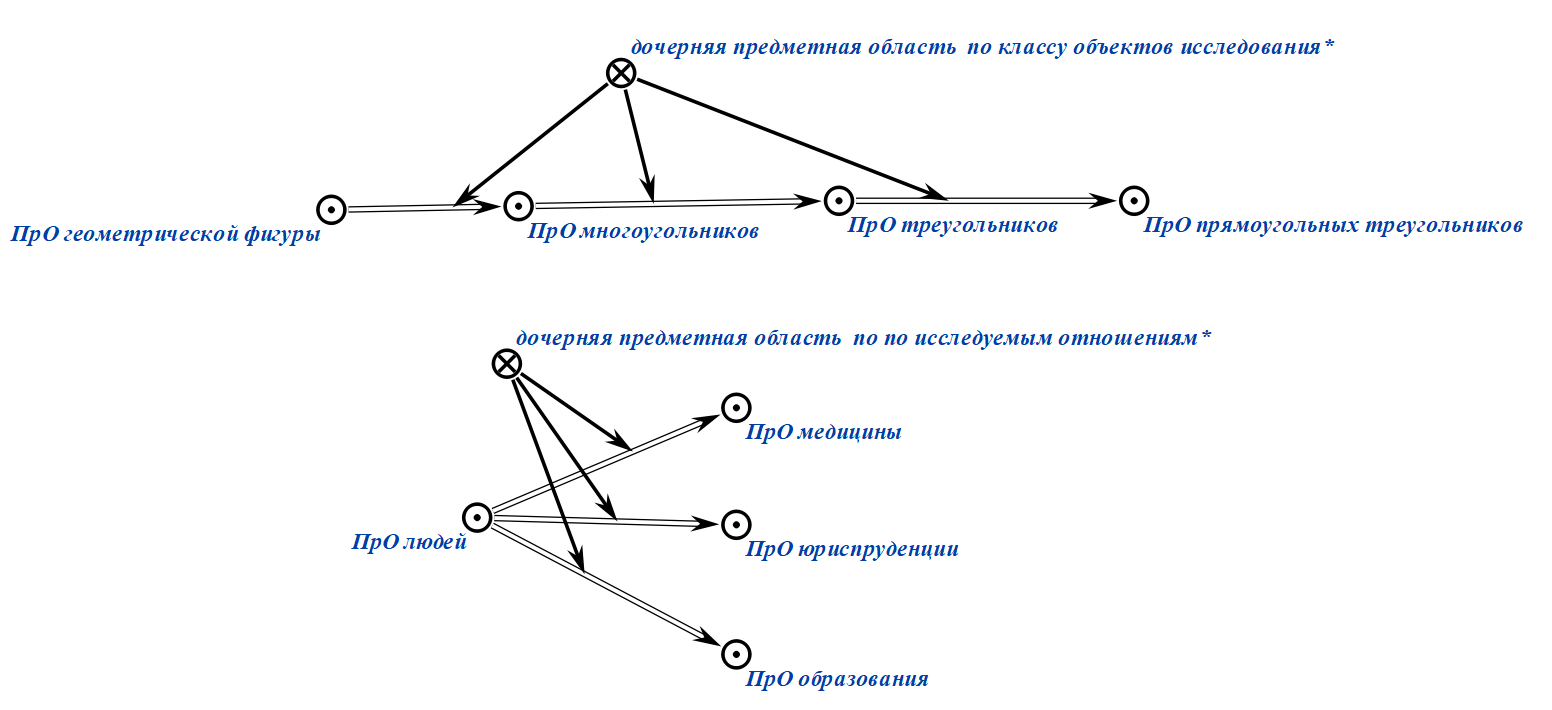
\includegraphics[scale=0.3]{./part1/pictures/example.png}
		\caption{Пример дочерних областей}
	\end{figure}
\end{frame}

\begin{frame}{\\}
	\begin{figure}[H]
		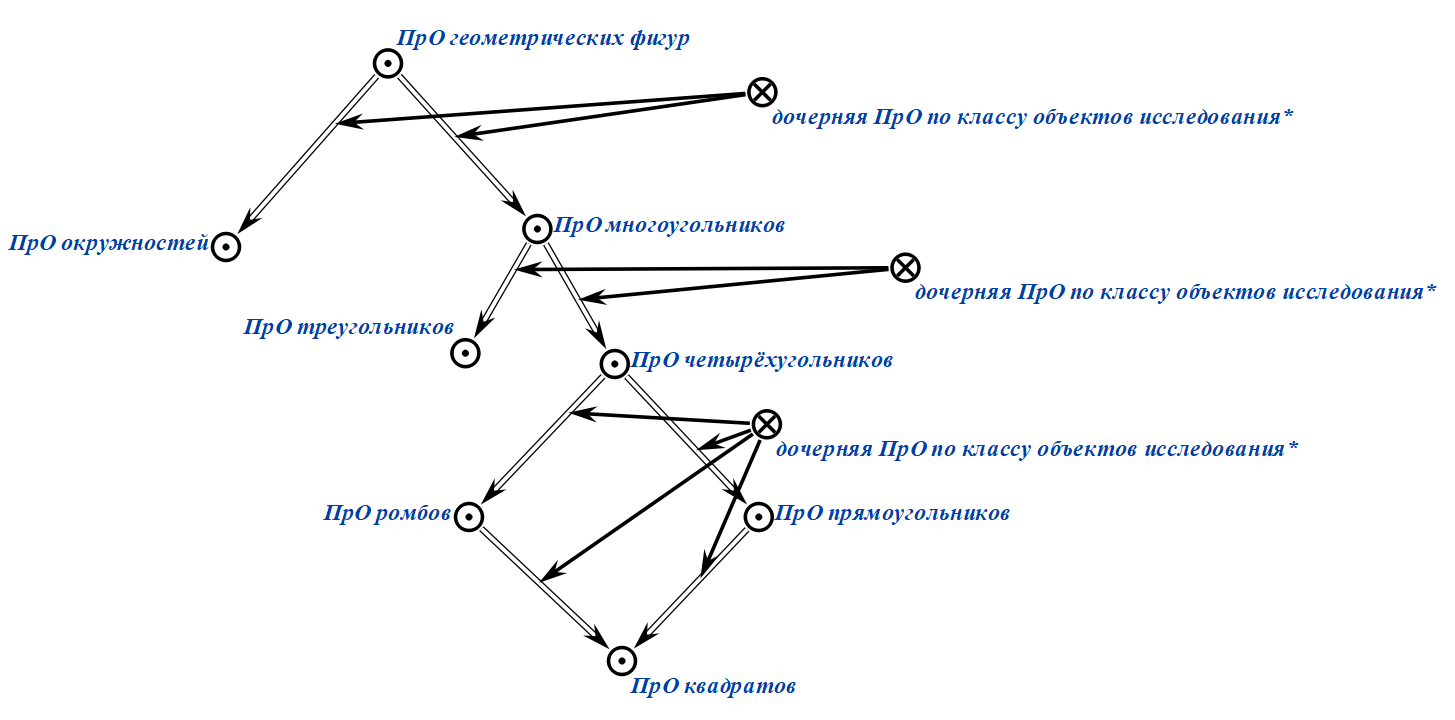
\includegraphics[scale=0.3]{./part1/pictures/inheritance.png}
		\caption{Пример наследования}
	\end{figure}
\end{frame}

\begin{frame}{\\}
	\begin{figure}[H]
		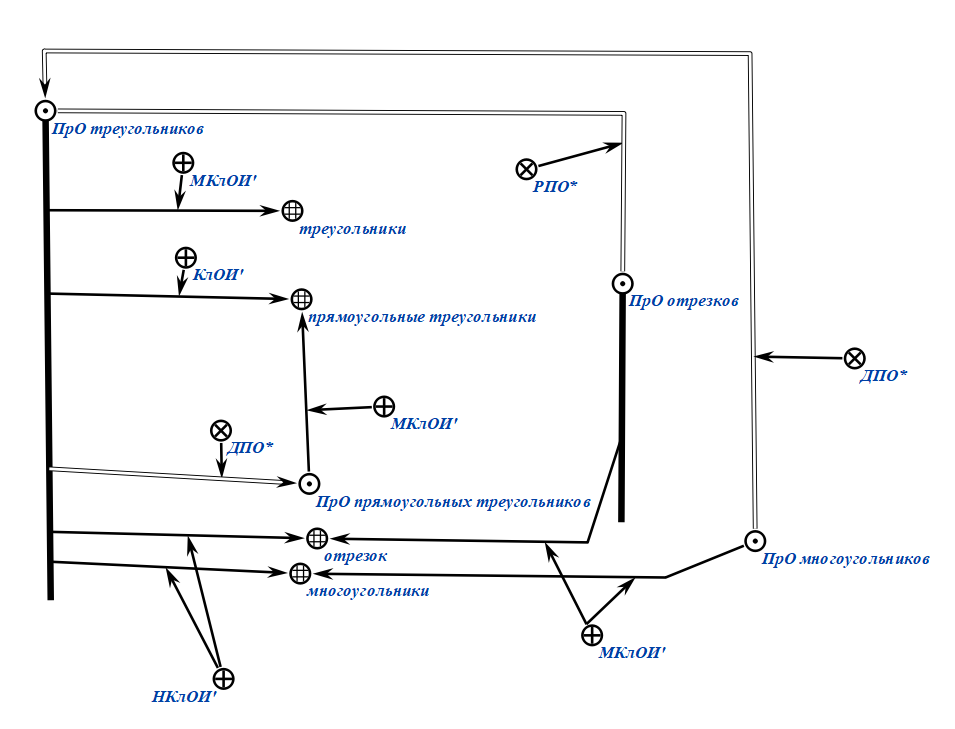
\includegraphics[scale=0.4]{./part1/pictures/RPO.png}
		\caption{Пример родственной ПрО}
	\end{figure}

\end{frame}